\documentclass[a4paper, 12pt]{article}
\usepackage[T1]{fontenc}
\usepackage[scale=1,angle=0,opacity=1,color=black!60]{background}
\usepackage{tikzpagenodes}
\usepackage{lastpage}
\usepackage{lmodern}
\usepackage{float}
\usepackage[textwidth=420pt,textheight=630pt]{geometry}
\setlength{\oddsidemargin}{15.5pt}
%\usepackage[none]{hyphenat} %no cortar palabras
\usepackage{url}
\usepackage{amsmath}
\usepackage{hyperref}

\usepackage[spanish, activeacute]{babel} %Definir idioma español
\usepackage[utf8]{inputenc} %Codificacion utf-8
\backgroundsetup{contents={}} %Saca el 'draft'

\def\labelitemi{$\bullet$}

\begin{document}
	% TÍTULO, AUTORES Y FECHA
	\begin{titlepage}
		\vspace*{\fill}
		\begin{center}
			\Huge Shared Server: Definición de Arquitectura \\
			\bigskip\bigskip\bigskip
			
		\end{center}
		\vspace*{\fill}
	\end{titlepage}
	\pagenumbering{arabic}
	\newpage

	% ÍNDICE
	\tableofcontents
	\newpage
	%\pagenumbering{arabic}

	\section{Definición de Arquitectura}
	La arquitectura del Shared Server consite en un servidor NodeJS, implementado con el framework Express. Este servidor se conectará a una Base de Datos PostgreSQL.\\
	
	El servidor implementa una API REST\footnote{\url{https://github.com/DamiCassinotti/SharedServer-Taller2/blob/master/api/documentacion.yaml}}, la cual serrá utilizada tanto por una aplicación web (Backoffice) como por los Application Servers. Por otro lado, el Shared Server deberá conocer el estado de los diferentes Application Servers existentes, para lo cual deberán ser dados de alta previamente.
	
	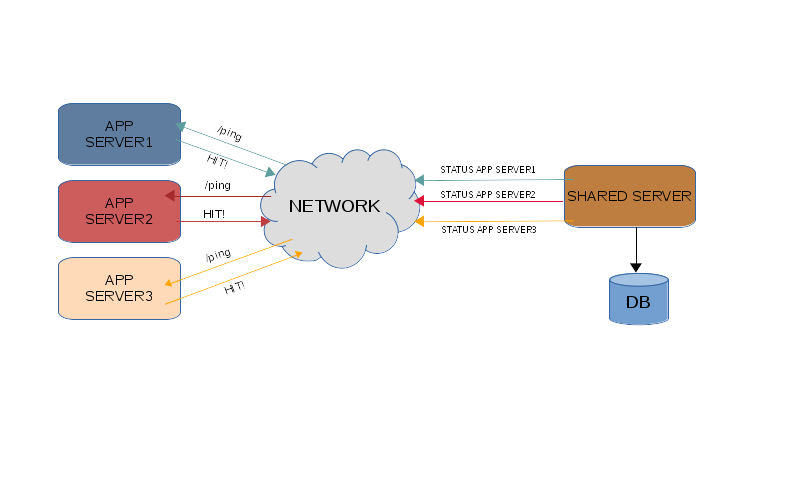
\includegraphics[width=\linewidth]{shared_server.png}
	
	Por otro lado, el servicio de autenticación utilizado para los servicios expuestos es JWT. El login de Backoffice es un login tradicional, mediante usuario y contraseña, que devuelve un token temporal que dará acceso a los distintos servicios. En cambio, la identificación de los App Servers se realiza de la siguiente manera:
	
	\begin{itemize}
	\item El App Server se da de alta, enviando su URL.
	\item El Shared Server da de alta al servidor en la base de datos. Devuelve una clave secreta (token sin expiración)
	\item El App Server guarda dicha clave, y la utiliza como llave para poder resetear su token temporal.
	\item Una vez obtenido el token temporal, se utiliza hasta su expiración para consumir los servicios del Shared Server
	\end{itemize}
	
	Por último, la base de datos relacional utilizada es PostgreSQL. En ella se guardan todos los datos referentes a los envíos, pagos, servidores, etc.

	\section{Diseño de aplicación}
	El diseño de la aplicación cuenta con tres capas principales:
	
	\begin{itemize}
	\item Routers: Son los encargados de proveer el enrutamiento de la aplicación. Además validan que los datos recibidos sean los correctos (en cuanto a obligatoriedad o tipos de datos). Manejan todo lo referido a los Requests y Responses. Se comunican con los controllers.
	\item Controllers: Los controllers reciben los datos de los routers; realizan las distintas validaciones de negocio necesarias (existencia de ids, etc); realizan los llamados a los services, y por último transforman los datos obtenidos de los services a modelos de negocio listos para enviar al cliente.
	\item Services: Los services son los encargados de ejecutar los queries a la DB. Estos reciben los datos validados, por lo que no deberían ocurrir errores de persistencia de datos. Además devuelven los datos tal cual fueron obtenidos desde las tablas.
	\end{itemize}
	
	Por otro lado, también se cuenta con otras clases auxiliares, como lo son los Validators o los Utils (estos últimos realizan las transformaciones de objetos de negocio).\\
	
	Realizar esta modularización permitió realizar un testeo más sencillo, ya que cada capa tiene su comportamiento bien diferenciado de las demás.
	

\end{document}
